\subsection{Dojo Funktion}
Die Funktionalitäten wurden von der Auftraggeberin Jana Kalbermatten ausgearbeitet. In diesem Abschnitt werden die alltäglichen Bedienungsfunktionen erklährt. Es wird dabei in Grundsätzlich drei Funtionsmodi unterteilt, die nachfolgend genauer erläutert werden.
\subsubsection{Modus Dojo laden}
Zum laden wird der Dojo an eine Spetzielle Ladevorrichtung oder eine ladestation angeschlossen. Dabei wird ein Mikro-USB Kabel de Ladestation an den Dojo angeschlossen. Diese Ladestationen können auch problemlos als Stationen mit Steckplätzen für mehrere Dojos realisiert werden.
\subsubsection{Modus Ausstellung laden}
Vor der Eröffnung einer neuen Ausstellungen müssen die Audiodateien auf den Dojo geladden werden. Dies geschieht, mit dem Verbinden des Dojos auf einen Computer mittels Mikro-USB Kabel. Die SD Karte auf dem Dojo wird dadurch im Dateiverzeichniss des Computers sichtbahr. Durch unsere Java Applikation kann eine Ausstellung mit den verschiedenen Audiodateien zusammengestellt und die entsprechenden Beacon ID's und der entsprechenden Sprache gesetzt werden. Durch drücken des Buttons USB-Übertragung werden die Audiodateien automatisch mit der richtigen konfiguration auf den Dojo geladen.

\subsubsection{Modus Sprach- und Zutittsrechte laden}
Die Zutritts- und die Sprachinformationen werden beim Start des Museumsbesuch durch den Rezeptionisten auf den Dojo geladen. Diese Übertragung funktioniert drahtlos über Bluetooth. Zur Vorführzwecken haben wir diese Funktion ebenfalls in unsere Java Applikation eingefügt. Der Rezeptionist kann anhand des Besuchers die Zutrittsrechte und die Sprache bestimmen und diese Informationen drahtlos an den Dojo übertragen.

\subsubsection{Modus Rundgang}
Während dem Rundgang hat der Dojo 2 Funktionen. Die Hauptfunktion ist dabei das Abspielen der Kunstinformationen vor einem Objekt. Wenn der Besucher mit dem Dojo in die Nähre eines Objektes kommt, fibriert der Dojo kurz, um dem Besucher das vorhandenseins einer Audiodatei zu signalisieren. Drückt der Besucher den Play Button, wird die Audiodatei der letzten Vibration abgespielt.Die Audiodatei kann durch den Knochenschallgeber, wercher sich am oberen Ende des Dojos befindet abgehört werden. Durch betätigen der Lauter-und der Leiser Taste kann die Lautstärke varriert werden. Wenn der Besucher ein zweites Mal den Play-Button betätigt, wird die Audiodatei pausiert, und kann durch ein weiteres mal betätigen wieder fortgesetzt werden. Wird nach dem Pausieren das Objekt gewechselt, signalisiert der Dojo das Vorhandenseins einer weiteren Audiodatei und diese wird zum Abspielen forbereitet. Der Fortschritt der Pausieren Audiodatei wird dabei nicht gespeichert. Wenn der Besucher vor einem Objekt steht, und es besonders interessant findet, und später noch weitere Informationen darüber erhalten möchte, kann er den Like Button betätigen. Der Like Butten speichert die ID des Beacons auf dem Dojo ab. Nach dem Besuch kann der Dojo kabellos über eine Bluetoothverbindung mit einer Besucherkonsole verbunden werden. Der Dojo sendet die gelikten ID's an die Konsole, welche weitere Nützliche Informatioen für den Besucher bereitstellen kann. Nach korrektem Übertragen werden die ID-Daten auf dem Dojo gelöscht.
Eine weitere Funktion, die wir in unseren Prototypen eingebaut haben ist die Zugnagsberechtigung. Bei einem Durchgang, der verschlodden ist, kann der Dojo, ähnlich wie ein Badge an eine Konsole gehalten werden. Der Dojo stellt automatisch eine Verbindung mit der Türkonsole her, und vergleicht seine Berechtigungen mit dem Durchgang. Wurde die Berechtigung bei der Rezeption erteilt, wird der Durchgang erlaubt, und die Türe öffnet sich. Diese Funktion kann beispielsweise beim Haupteingang nach der Rezeption mit einem Drehkreuz verwendet werden, oder bei mehreren Ausstellungen in verschiedenen Räumen.
\clearpage
\subsection{Dojo Aufbau}
Das Design des Dojos aus Abbildung \ref{fig:DojoBild} wurde für die Batcherorarbeit von Jana Kalbermatten erarbeitet und dient als Vorlage für das Gerät. Der Dojo ist mit $245mm$ ziemlich lang, besitzt jedoch mit einem Aussendurchmesser von nur $19.5mm$ einen kleinen Querschnitt. Dieses Gehäuse setzt eine detailierte Planung der elektronischen Bauteile voraus, sowie ein kompaktes Design der elektronischen Schaltung.


\begin{figure}[h]
	\centering
	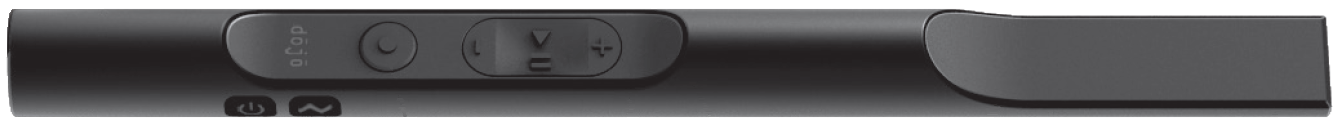
\includegraphics[width=\textwidth]{graphics/DojoBild.png}
	\caption{Aussenansicht des Dojos}
	\label{fig:DojoBild}
\end{figure}

Durch den begrenzten Durchmesser und der begrenzten Schiebeöffnung auf der Rückseite des Dojos kommen keine Akkumulatoren der Normgrösse $A$ sowie $AA$ infrage. Eingebaut wird daher ein Akkumulator der Grösse $AAA$. Um mit den Tastern und dem USB-Port nicht in konflikt zu geraten, wird der Akkumulator in der Mitte des Dojos eingebaut siehe Abbildung \ref{fig:DojoQuerschnitt}. Dies hat ebenfalls den Vorteil, das man einen Print der Länge $120mm$ einbauen kann, der den USB Port, sowie alle Taster beinhaltet.

\begin{figure}[h]
	\centering
	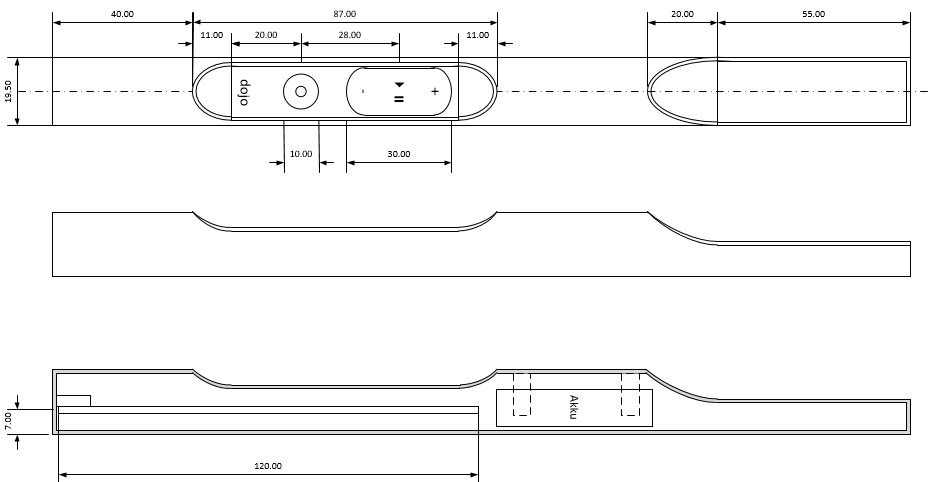
\includegraphics[width=\textwidth]{graphics/DojoQuerschnitt.png}
	\caption{Technische Zeichnung des Dojos}
	\label{fig:DojoQuerschnitt}
\end{figure}

\newpage

Der Akkumulator wird mit einer Stahl Batteriehalterung in das Gehäuse verbaut. Dabei bleibt, wie in der Abbildung \ref{fig:DojoAkkumulatorQuerschnitt} zu sehen, neben der Halterung genügend Platz für die Verbindungskabel, die zum Knochenschallgeber im Kopf des Dojos führen. Ebenfalls kann der Akkumulator durch den Schiebeöffner an der Rückseite des Dojos entfernt werden.

\begin{figure}[h]
	\centering
	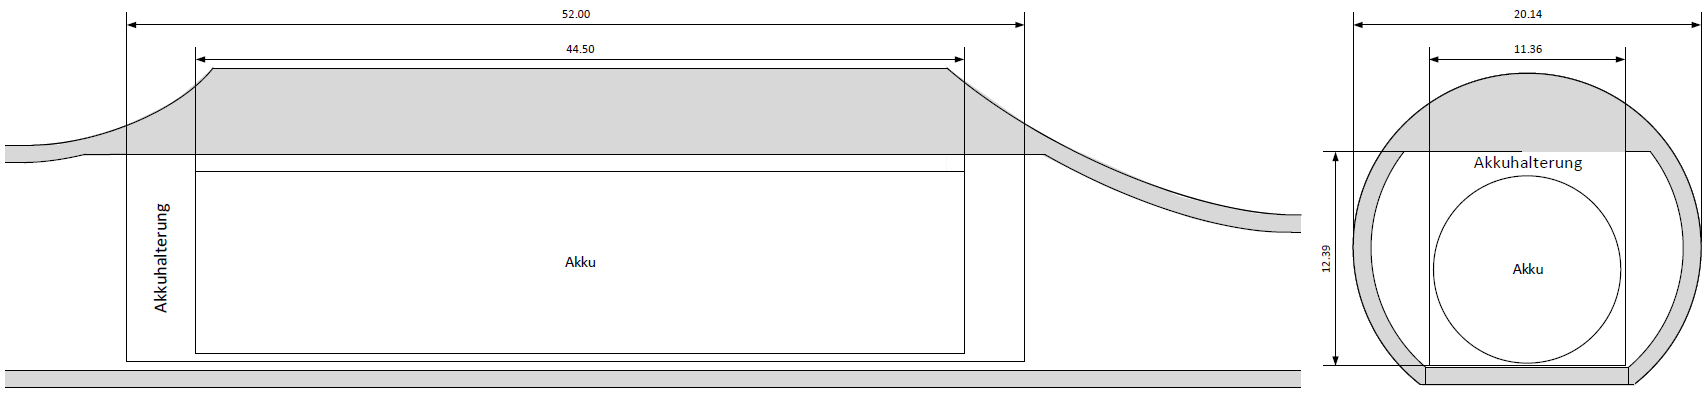
\includegraphics[width=\textwidth]{graphics/DojoAkkumulatorQuerschnitt.png}
	\caption{Positionierung des Akkumulators}
	\label{fig:DojoAkkumulatorQuerschnitt}
\end{figure}

Der Print nimmt mit einer Länge von $120mm$ und einer Breite von $17mm$ den grössten Teil des Gehäuses in Beschlag. Aufgrund der hohen Komplexität der elektronischen Schaltung handelt es sich um einen mehrlagigen Print. Am unteren Ende des Dojos befindet sich die Buchse der USB-Verbindung. Diese wird, wie in Abbildung \ref{fig:DojoPrintQuerschnitt} dargestellt, auf dem Print motiert. Die zweite Darstellung zeigt einen Querschnitt des Dojos bei den Tasten. Diese können auf dem Print montiert und mechanisch mit den Tastern des Gehäuses verbunden werden. Am Oberen Ende des Prints werden die Kontakte für die Batterie, sowie den Knochenschallgeber angebracht.

\begin{figure}[h]
	\centering
	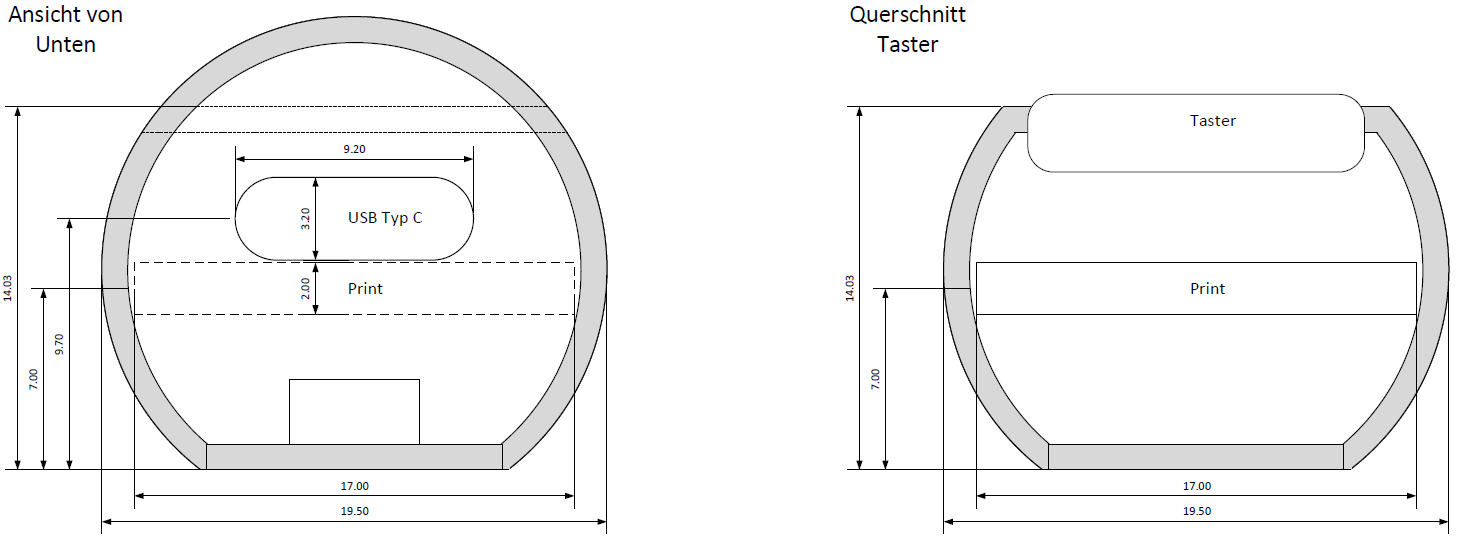
\includegraphics[width=\textwidth]{graphics/DojoPrintQuerschnitt.png}
	\caption{Positionierung des Prints}
	\label{fig:DojoPrintQuerschnitt}
\end{figure}


